GoにはRESTに対する直接のサポートはありません。しかし、RESTfulなwebアプリケーションはHTTPプロトコルに基づいて実装されるものですので、\texttt{net/http}パッケージを利用することで自分で実装することができます。当然RESTに対していくつか改造を行う必要があります。RESTは異なるmethodによって対応するリソースを処理します。現在すでに存在する多くの自称RESTアプリケーションは、実は本当にRESTを実装しているわけではありません。ここではとりあえずこれらのアプリケーションを実装しているメソッドにしたがっていくつかのレベルに分けてみます、以下の図をご覧ください:



\begin{figure}[H]
   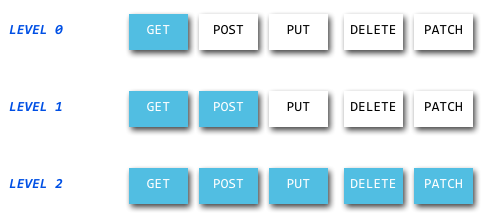
\includegraphics[width=14cm]{8.3.rest3.png}
   \label{図8.7}
   \caption{RESTのレベル分け}
\end{figure}


上の図は我々が現在実装しているRESTの3つのlevelを示しています。我々がアプリケーションを開発する時も必ずしも全てのRESTfulのルールをまるっとその方式を実装しているわけではありません。なぜならある時はRESTfulの方式を完全に参照しなくても大丈夫だからです。RESTfulサービスは\texttt{DELETE}と\texttt{PUT}を含む各HTTPの方法を十分に利用します。しかしある時は、HTTPクライアントは\texttt{GET}と\texttt{POST}リクエストのみを送信できます:

\begin{itemize}
  \item HTML標準はリンクとフォームを通してのみ\texttt{GET}と\texttt{POST}をサポートしています。Ajaxをサポートしていないウェブブラウザでは\texttt{PUT}や\texttt{DELETE}コマンドを送信することはできません。
  \item あるファイアウォールはHTTPの\texttt{PUT}と\texttt{DELETE}リクエスト遮ることがあり、この制限を迂回するにはクライアントの実際の\texttt{PUT}と\texttt{DELETE}リクエストをPOSTリクエストから通していかなくてはなりません。そのためRESTfulサービスは受け取ったPOSTリクエストからオリジナルのHTTPメソッドを探し出す方法と元に戻す方法を行う責任があります。
\end{itemize}

現在\texttt{POST}の中において隠されたフィールドである\texttt{\_method}を増加するなどの方法で\texttt{PUT}、\texttt{DELETE}といったメソッドをエミュレートすることができます。しかし、サーバでは変換を行う必要があります。現在私のプロジェクトではこのような方法によってRESTインターフェースを作成しています。当然Go言語では完全にRESTfulに沿った実装を行うのは容易です。下の例を通してどのようにRESTfulなアプリケーションの設計を実現するかご説明しましょう。

\begin{lstlisting}[numbers=none]
package main

import (
    "fmt"
    "github.com/julienschmidt/httprouter"
    "log"
    "net/http"
)

func Index(w http.ResponseWriter, r *http.Request, _ httprouter.Params) {
    fmt.Fprint(w, "Welcome!\n")
}

func Hello(w http.ResponseWriter, r *http.Request, ps httprouter.Params) {
    fmt.Fprintf(w, "hello, %s!\n", ps.ByName("name"))
}

func getuser(w http.ResponseWriter, r *http.Request, ps httprouter.Params) {
    uid := ps.ByName("uid")
    fmt.Fprintf(w, "you are get user %s", uid)
}

func modifyuser(w http.ResponseWriter, r *http.Request, ps httprouter.Params) {
    uid := ps.ByName("uid")
    fmt.Fprintf(w, "you are modify user %s", uid)
}

func deleteuser(w http.ResponseWriter, r *http.Request, ps httprouter.Params) {
    uid := ps.ByName("uid")
    fmt.Fprintf(w, "you are delete user %s", uid)
}

func adduser(w http.ResponseWriter, r *http.Request, ps httprouter.Params) {
    // uid := r.FormValue("uid")
    uid := ps.ByName("uid")
    fmt.Fprintf(w, "you are add user %s", uid)
}

func main() {
    router := httprouter.New()
    router.GET("/", Index)
    router.GET("/hello/:name", Hello)

    router.GET("/user/:uid", getuser)
    router.POST("/adduser/:uid", adduser)
    router.DELETE("/deluser/:uid", deleteuser)
    router.PUT("/moduser/:uid", modifyuser)

    log.Fatal(http.ListenAndServe(":8080", router))
}
\end{lstlisting}

上のコードではどのようにRESTなアプリケーションを書くかご覧いただきました。我々がアクセスするリソースはユーザです。異なるmethodによって異なる関数にアクセスしました。ここではサードパーティライブラリgithub.com/julienschmidt/httprouterを使用しています。前の章でどのように自分で定義したルータを実現するかご紹介しました。このライブラリは自分で定義したルートと便利なルートのルールを反映させます。これを使って簡単にRESTのフレームワークを実装することができます。
